\documentclass[10pt,a4paper]{article}
\usepackage[utf8]{inputenc}
\usepackage[english]{babel}
\usepackage[left=2cm,right=2cm,top=2cm,bottom=2cm]{geometry}
\usepackage[hyphens]{url}
\usepackage{hyperref}
\usepackage{listings}
\usepackage{amsmath}
\usepackage{amsfonts}
\usepackage{amssymb}
\usepackage{color}
\usepackage{graphicx}
\graphicspath{{Figures/}}
\author{Pierre Lecomte \\ \textit{ \href{mailto:pierre.lecomte@gadz.org}{pierre.lecomte@gadz.org}}}
\title{ambitools Documentation}

%%% MY COLORS
\definecolor{yoheader}{rgb}{0.71,0.01,0.0}

%%%% margin par
\definecolor{margincolor}{rgb}{0.52,0.02,0.02} % grey red.
\definecolor{yobg}{rgb}{0.9,0.9,1}
\definecolor{yotxt}{rgb}{0.01,0.01,0.52}
\definecolor{mylstcmt}{rgb}{0.01,0.52,0.01} % a dark green.
%\definecolor{mylstdoc}{rgb}{0.60,0.60,0.60} % a medium grey.
\definecolor{mylstdoc}{rgb}{0.80,0.30,0.80} % a medium pink.
%\definecolor{mylsteqn}{rgb}{0.80,0.80,0.30} % a medium pink.
\definecolor{mylstkey}{rgb}{0.52,0.01,0.01} % a dark red.
%%\newcommand{\farg}[1]{\textrm{\textit{#1}}}

\begin{document}

\lstset{
  tabsize=4,
  showspaces=false,
  showstringspaces=false,
  %language=C++, 
  basicstyle=\ttfamily\color{yotxt},
  numbers=none,
  stepnumber=2,
  commentstyle=\slshape\color{mylstcmt},
  breaklines=true, 
  emph={Gain,Radius,Azimuth,Elevation,Spherical, Wave, Speakers,Mute,NFC,Outputs,Inputs},
  emphstyle=\color{mylstkey},
%  morecomment=[s][\color{mylsteqn}]{<equation>}{</equation>},
  morecomment=[s][\color{mylstdoc}]{<mdoc>}{</mdoc>},
  %% frame=single,
  backgroundcolor=\color{yobg},
  captionpos=b
}

\makeatletter
\newcommand\footnoteref[1]{\protected@xdef\@thefnmark{\ref{#1}}\@footnotemark}
\makeatother

\maketitle
\tableofcontents
\section{Introduction}

\subsection{Goals of ambitools}
ambitools is a collection of tools for sound-field synthesis using Near-Field Compensated Higher Orders Ambisonics (NFC-HOA). For the rest of this document, the denomination Ambisonics will be used for simplicity.
ambitools is developped in the context of my PhD on 3D sound field synthesis. The audio processing is coded in \textsc{Faust}\footnoteref{faustlive} (Functional AUdio Stream) which allows to produce efficent C++ code and exports in various DSP tools format : VST, standalone applications, LV2, etc. Thus, ambitools is multi-platform (although conceived under Linux/Jack).

The goal of ambitools is mainly to produces several modules to encode, decode and transform 3D synthesized sound field or 3D recordings in a context of physical sound field synthesis. 

The project is open-source under GPL licence. ambitools is thought to be very flexible to adapt to your configuration. The \textsc{Faust}-code for each tools has an header with the required order. So, for example, if you need an encoder up to order $M=4$, for $N=5$ sources, you just has to change this two parameters in \lstinline'hoa_encoder_N_sources.dsp' and produce de required plug-in using \textsc{FaustLive}\footnote{\label{faustlive}\url{http://faust.grame.fr}} for example.

Don't hesitate to contact me for any suggestions, requirements, critics or even just to tell me you're using ambitools !

\begin{flushright}
Pierre Lecomte
\end{flushright}

\subsection{Ambisonics with ambitools overview}
This section presents the basis of Ambisonics for 3D sound field synthesis. It is written with relatively few maths to focus on the concepts instead of the mathematical rigor, which would be out of scope of this document. If you want more insights to Ambisonics refer for example to \cite{daniel2000representation,poletti2005three,ahrens2012analytic}.

\subsubsection{Principles}
Ambisonics are some mathematical approaches to represent a sound field in two or three dimensions over a basis of spherical harmonics. Without giving more mathematical details, Ambisonic main possibilities are displayed on Fig.~\ref{fig:ambisonics}.
\begin{figure}[!ht]
	\centering
	\def\svgwidth{\columnwidth}
	\input{Figures/Fig_Apercu_Ambisonics.pdf_tex}
	\caption{Ambisonic principles: A sound field can be captured in three dimensions using spherical microphone or it can be synthesized with monophonic signals and explicit positions in space. These two approaches result in an encoded sound field in Ambisonic domain up to order $M$. In this domain, transformations can be done such as: sound field mirroring, rotation, warping, directional filtering, etc. Finally, the decoding step computes the driving signals of the playback loudspeakers to recreate the encoded sound field in a sweet spot region of space. The decoding can be done over various configurations of speakers and even over headphones !}
	\label{fig:ambisonics}
\end{figure}

Thus, in accordance to this Fig.~\ref{fig:ambisonics}, ambitools provides tools to:
\begin{itemize}
\item Encode a sound field captured by spherical microphone.
\item Encode a sound field from monophonic signals and explicit position in space.
\item Transform and manipulate the encoded sound field in Ambisonic domain.
\item Decode the sound field over spherical grids of speaker or over headphones with binaural convolution.
\end{itemize}

\subsubsection{Spherical coordinate system}
Ambisonics are usually described in spherical coordinate systems. In ambitools, the following spherical coordinate system is used:
The following spherical coordinate system is used and is shown in Fig.~\ref{fig:coord_sph}:
\begin{equation}
x = r \cos(\theta) \cos(\delta), \; y = r \sin(\theta) \cos(\delta), \;
z = r \sin(\delta)\textcolor{red}{.}
\end{equation}
\begin{figure}[ht]
\centering
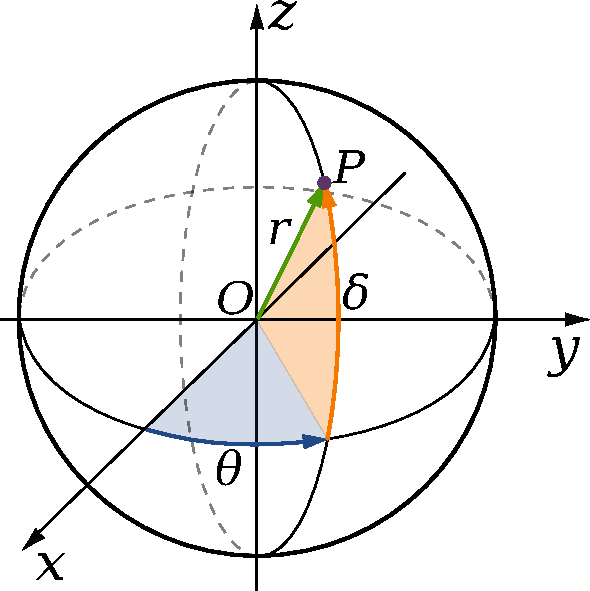
\includegraphics[height=0.3\columnwidth]{Fig_Coord_Sph.pdf}
\caption{Spherical coordinate system in use. A point $P (x,y,z)$ is described by radius $r$, azimuth $\theta$ and elevation $\delta$.}
\label{fig:coord_sph}
\end{figure}
The azimuth angle $\theta \in [0~~360^\circ]$. The elevation angle $\delta \in [-90^\circ~~90^\circ]$.

\subsubsection{Spherical harmonics}
As mentionned before, Ambisonics describes a sound field over a spherical harmonics basis. Those functions are directional functions of the variable $\theta,\delta$. They are denoted $Y_{mn}(\theta,\delta)$ where subscript $m$ represent the order of the spherical harmonic and $n$ its degree. There is several definition for these functions. In ambitools, the N3D real spherical harmonic definition is used \cite{daniel2000representation}:
\begin{multline}
Y_{mn}(\theta,\delta) = \sqrt{(2m+1)\epsilon_n \frac{(m-|n|)!}{(m+|n|)!}} P_{m|n|}(\sin(\delta)) \\
 \times \left\lbrace \begin{aligned} \cos(|n| \theta) & & \text{if} & & n \geq 0 \\ \sin(|n| \theta)  & & \text{if} & & n < 0  \end{aligned} \right.,
\label{eq:ymn}
\end{multline}
where $P_{m|n|}$ are the associated Legendre polynomials of order $m$ and degree $|n|$, $(m,n) \in (\mathbb{N},\mathbb{Z})$ with $|n| \leq m$, and $\epsilon_n = 1$ if $n = 0$, $\epsilon_n = 2$ if $|n| > 0$. In Eq.~\eqref{eq:ymn}, $m$ denotes the spherical harmonic order and $n$ its degree.

For each order $m$, there are $(2 m +1)$ spherical harmonics. Thus a basis truncated at order $M$ contains $(M+1)^2$ functions. For example, on Fig.~\ref{fig:spherical_harmonics} are displayed the spherical harmonics up to order $M=5$ as balloon plots.

Thus, a sound field can be described as a linear combination of spherical harmonics. The weights of this linear combination are called the Ambisonics components or $B$-Format components. As an example, a sound field described up to order $M=1$ is described with $(M+1)^2=4$ Ambisonics components. At order $M=5$ there will be $36$ components, etc.

Without giving more details, the concept to retain is that the more components are available to describe the sound field (i.e. the higher the order), the larger the sweet-spot will be on Fig.~\ref{fig:ambisonics}.

At the moment, ambitools offers the possibility of 3D Ambisonics up to order $M=5$. Thus for all the tools you need to compile, \textcolor{red}{\textsc{$M$ should be chosen such as $M \leq 5$.}}

\begin{figure}[ht]
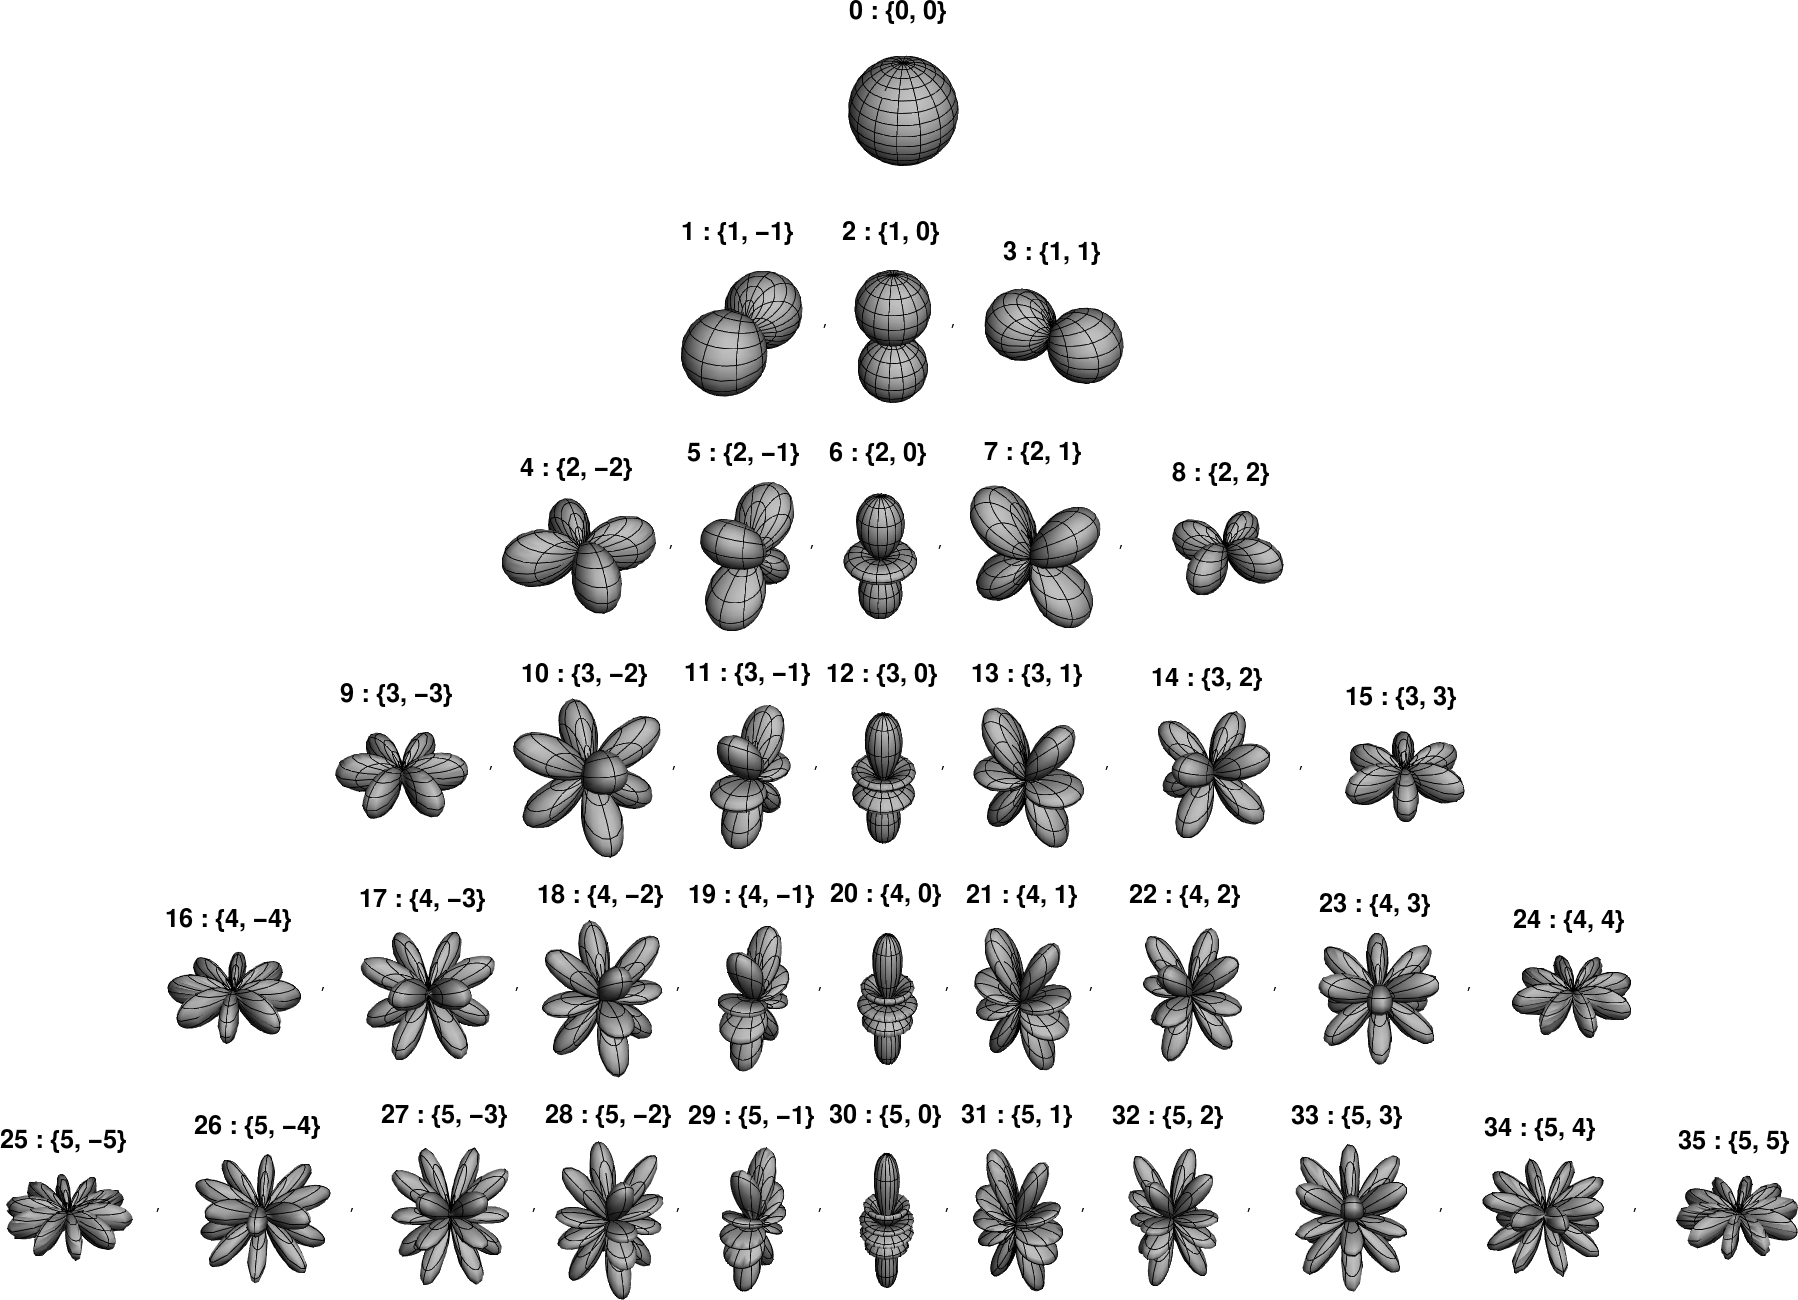
\includegraphics[width=\columnwidth]{Fig_YACN.png}
\caption{Balloon-plot of the spherical harmonics up to order $M=5$.}
\label{fig:spherical_harmonics}
\end{figure}

\pagebreak
\section{Installing ambitools}

\subsection{Retrieve ambitools repository}
To install ambitools, simply go on the github repository\footnote{\url{https://github.com/sekisushai/ambitools}} and clone it. To do so, open a terminal in the directory you'd like to clone the repository and type the following command:

\begin{lstlisting}
$ git clone https://github.com/sekisushai/ambitools
\end{lstlisting}

To keep the repository up to date, type the following command at the root of the directory \lstinline`ambitools/`:

\begin{lstlisting}
$ git pull
\end{lstlisting}

You can also download a \lstinline'.zip' file from github\footnote{\url{https://github.com/sekisushai/ambitools/archive/master.zip}}

The resulting \lstinline'ambitools/' folder should have the following structure:

\begin{itemize}
    \item \lstinline'Documentation/' Everything concerning the documentation (pdfs, including some scientific papers).
    \item \lstinline'Faust/' Everything written in \textsc{Faust} language (all the ambitools plug-ins + some utilities).
    	\subitem \lstinline'bin/' Compiled plug-ins in various formats.
    	\subitem \lstinline'src/' Source code of the plug-ins.
    	\subitem \lstinline'src/lib/' Shared libraries (spherical harmonics, gui, etc.).
    \item \lstinline'FIR/' Finite Impulse Response (FIR) filters banks for binaural rendering and spherical microphone equalization filters, to use with Jconvoler\footnote{\url{http://kokkinizita.linuxaudio.org/linuxaudio/}}, fast convolution software.
    	\subitem \lstinline'spherical_microphones/' Equalization filters for rigid spherical microphone, such as mh acoustics EigenMike\textsuperscript{\textregistered}\footnote{\url{http://www.mhacoustics.com}}
  		\subitem \lstinline'hrir/' Head Related Impulses Responses (HRIR) of several people to use with binaural rendering over headphones.
    \item \lstinline'Processing/' Everything written in \textsc{Processing} language, namely the spherical VU-Meter ((see Sec.~\ref{sec:processing}).
    	 \subitem \lstinline'bin/' Compiled spherical VU-Meter in Java for various architectures.
    	 \subitem \lstinline'src/' \textsc{Processing} source code.
    \item \lstinline'PureData/' Everything written in Pure Data (a few sounds generator patches, head-tracking patch and PlayStation-like remote patch to drive \textsc{Faust} plug-ins with Open Sound Control protocol, OSC).
\end{itemize}

\subsection{Compile the \textsc{Faust} plug-ins}
The \textsc{Faust} plug-ins source codes are in the sub-folder \lstinline'Faust/src/'. 

\subsection{Local \textsc{Faust} installation}
If you have \textsc{Faust} installed on your machine with the required dependencies, you can run the scripts collection \lstinline'faust2*' to produce the plug-in of your choice in the desired format. 

For example, to compile \lstinline'hoa_encoder_N_sources.dsp' into a standalone Linux jack-qt application with \textsc{OSC} support, type the following command in a terminal in the folder \lstinline'\Faust/src'

\begin{lstlisting}
$ faust2jaqt hoa_encoder_N_sources.dsp -osc
\end{lstlisting}

\subsection{\textsc{FaustLive}}
To compile the plug-ins to your requirements, load the chosen plug-in in \textsc{FaustLive}\footnoteref{faustlive} and choose \lstinline'Window/Export As...' (see Fig.~\ref{fig:faustlive}).
\begin{figure}[!ht]
\centering
\includegraphics[width=0.3\columnwidth]{faustlive_export_manager.png}
\caption{\textsc{FaustLive} Export Manager}
\label{fig:faustlive}
\end{figure}

\subsection{Compile the \textsc{Processing} VU-Meter}
The \textsc{Processing} source code is in the folder \lstinline'Processing/scr'. You should open the file \lstinline'Spherical_VU_Meter.pde' in the \textsc{Processing} editor and select "File/Export..." to produce a binary application.

\section{The different tools}
This section gives a quick presentation of each tool contained in ambitools. 
\subsection{\textsc{Faust}}
The core of the sound processing is written in \textsc{Faust} language. Note that the majority of the figures presented here will be screenshots of the tools compiled as standalone \textsc{Jack} applications for Linux, using \lstinline'faust2jaqt' script. However, thanks to the versatility of \textsc{Faust} language, remember that each of these tools can be compiled for various architecture, using \textsc{FaustLive}\footnoteref{faustlive} for example. 

\pagebreak
\subsubsection{hoa\_N\_sources\_encoder}
\label{sec:hoa_encoder}
\begin{itemize}
\item Inputs: $N$
\item Outputs: $(M+1)^2$
\end{itemize}

This first tool allows to encode $N$ signal inputs to an 3D Ambisonics scene described with Ambisonics components signals up to order $M$ (the $B$-Format). You can choose $N$ and $M$ at the compilation time in file \lstinline'hoa_encoder_N_sources.dsp'. The resulting graphical user interface when using \lstinline'faust2jaqt' script is shown in Fig.~\ref{fig:hoa_encoder} for $N=3, M=5$.
Each input signal can be encoded in $B$-Format as a plane wave or a spherical wave. 

For the plane wave case, the check-box \lstinline'Spherical Wave' should be unchecked. Consequently, the knob \lstinline'Radius' and input entry \lstinline'Speakers Radius' are without effect in this case (a plane wave has no distance information).

For the spherical wave case, the knob \lstinline'Radius' allows to choose the source radius to origin. Note that to represent a spherical wave in Ambisonic domain, near-field filters are activated \cite{daniel2003spatial,lecomte2015real}. Those filters, unstable by nature, are stabilized using the near-field compensation filters from decoding step. Thus in this case, the radius of the spherical loudspeakers grid should be known prior to decoding and given in \lstinline'Speakers Radius' input entry.

Finally, the outputs of this tool are $B$-Format signals up to order $M$. Each order can be muted or each individual Ambisonic components individually.

\begin{figure}[!ht]
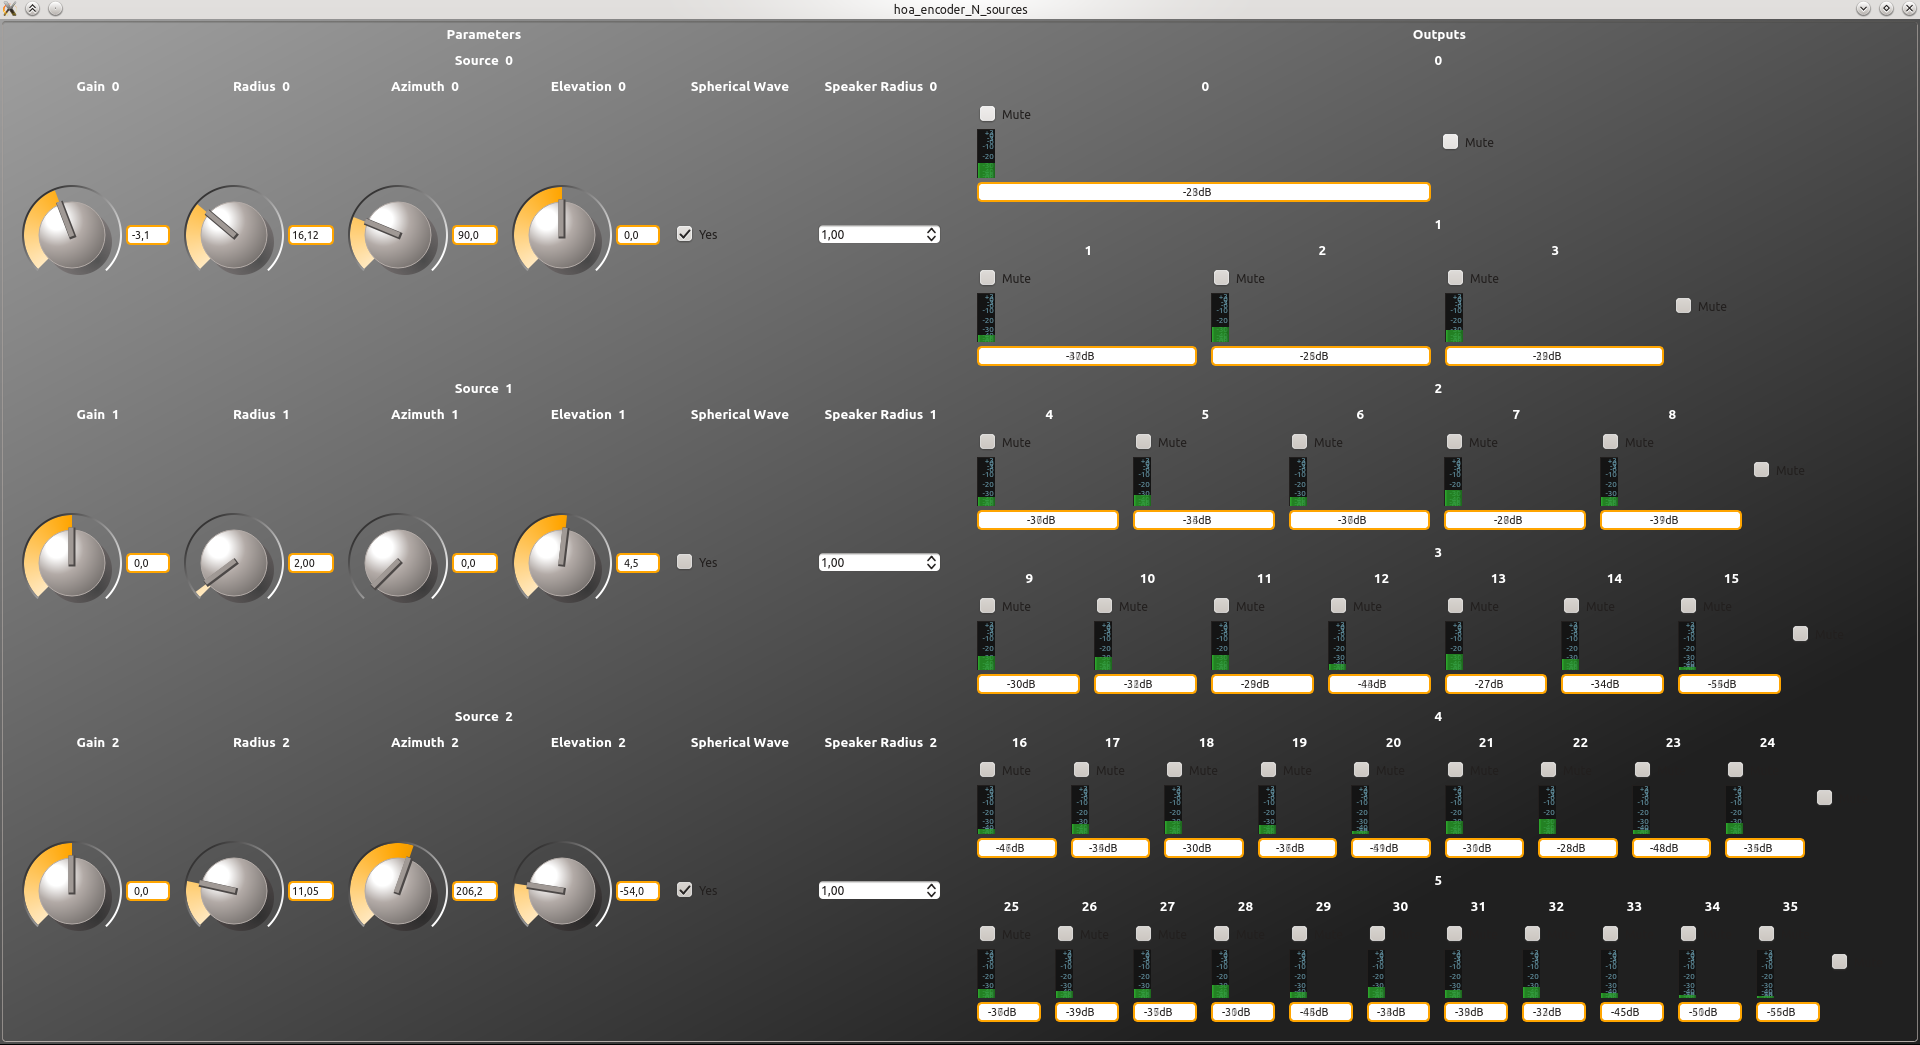
\includegraphics[width=\columnwidth]{hoa_encoder.png}
\caption{\lstinline'hoa_encoder_N_sources' plug-in compiled using \lstinline'faust2jaqt' script with $N=2$ and $M=5$. The \lstinline'Gain' knob allows to adjust the input level of the input. \lstinline'Radius' knob allows to choose the source distance to origin in case of spherical wave encoding. \lstinline'Azimuth' and \lstinline'Elevation' knobs allow to choose the source direction. The \lstinline'Spherical Wave' check-box enables the encoding of spherical wave, using near-field filters. \lstinline'Speakers Radius' sets the radius for the spherical arrays of loudspeakers at decoding stage in case of spherical wave encoding. Finally, the VU-Meters shows the level of 3D $B$-Format signals in dBFS up to order $M$. Each meter as a \lstinline'Mute' check-box and each order as well.}
\label{fig:hoa_encoder}
\end{figure}

\pagebreak
\subsubsection{hoa\_decoder\_*}
\label{sec:hoa_decoder}
\begin{itemize}
\item Inputs: $(M+1)^2$
\item Outputs: $26$ or $50$ depending on the decoder.
\end{itemize}

Two basic decoder by mode-matching \cite{daniel2000representation,poletti2005three} are available at the moment in ambitools: \lstinline'hoa_decoder_lebedev26' and
\lstinline'hoa_decoder_lebedev50'. Those two decoder allows to decode $(M+1)^2$ $B$-Format signals on Lebedev grids with respectively $26$ and $50$ loudspeakers \cite{lebedev1975values,lecomte2015on}. Those grids are able to reconstruct the sound field up to order $M=3$ and $M=5$ respectively.
If other decoder are required, you should have a look at the ambisonic decoder toolbox from Aaron Heller \cite{heller2012toolkit}, or contact me. The graphical user interface when using \lstinline'faust2jaqt' script is shown in Fig.~\ref{fig:hoa_decoder_lebedev50} for the \lstinline'hoa_decoder_lebedev50' decoder compiled with $M=5$. The decoder can be with or without near-field compensation (NFC) filters \cite{daniel2003further,lecomte2015real}. Those filters allow to take into account the finite distance of the loudspeakers: In other terms, if they are disabled, the loudspeakers are modeled as plane-wave generators. In case of spherical wave encoding using the \lstinline'hoa_N_sources_encoder' plug-in, the \lstinline'NFC' check-box should be unchecked as the near-field compensation filters are already used at encoding step (see Sec.~\ref{sec:hoa_encoder}).
\begin{figure}[!ht]
\includegraphics[width=\columnwidth]{hoa_decoder_lebedev50.png}
\caption{\lstinline'hoa_decoder_lebedev50' compiled using \lstinline'faust2jaqt' script with $M=5$. The slider \lstinline'Outputs Gain' apply a global gain on all outputs (loudspeakers signals). The slider \lstinline'Inputs Gain' apply a global gain on all inputs ($B$-Format signals). The VU-Meters \lstinline'Inputs' and \lstinline'Outputs' give the signals level in dBFS. The check-box \lstinline'NFC' activate or deactivate the near-field compensation filters. The input entry \lstinline'Speakers Radius' allows to set the spherical grid radius. Finally, the check-boxes \lstinline'Mute' above all inputs VU-meters allow to mute some specific $B$-Format signals. Or, all the signal from an order with \lstinline'Mute' check-boxes on side of an VU-Meter group.}
\label{fig:hoa_decoder_lebedev50}
\end{figure}

\pagebreak
\subsubsection{hoa\_panning\_*}
\label{section:hoa_panning}
\begin{itemize}
\item Inputs: $N$
\item Outputs: $26$ or $50$ depending on the configuration.
\end{itemize}

It is possible to compute directly the driving signals of the loudspeakers without passing by and encoding/decoding process \cite{lecomte2015on}. This equivalent 3D panning is implemented in the tools \lstinline'hoa_panning_lebedev26' and \lstinline'hoa_panning_lebedev50' for 26 and 50 loudspeakers Lebedev grids respectively.
The graphical user interface using \textsc{Faust} Linux jack-qt compiler is shown in Fig.~\ref{fig:hoa_panning_lebedev50} for the \lstinline'hoa_panning_lebedev50' tool. For this version, two spherical waves are synthesized.
\begin{figure}[!ht]
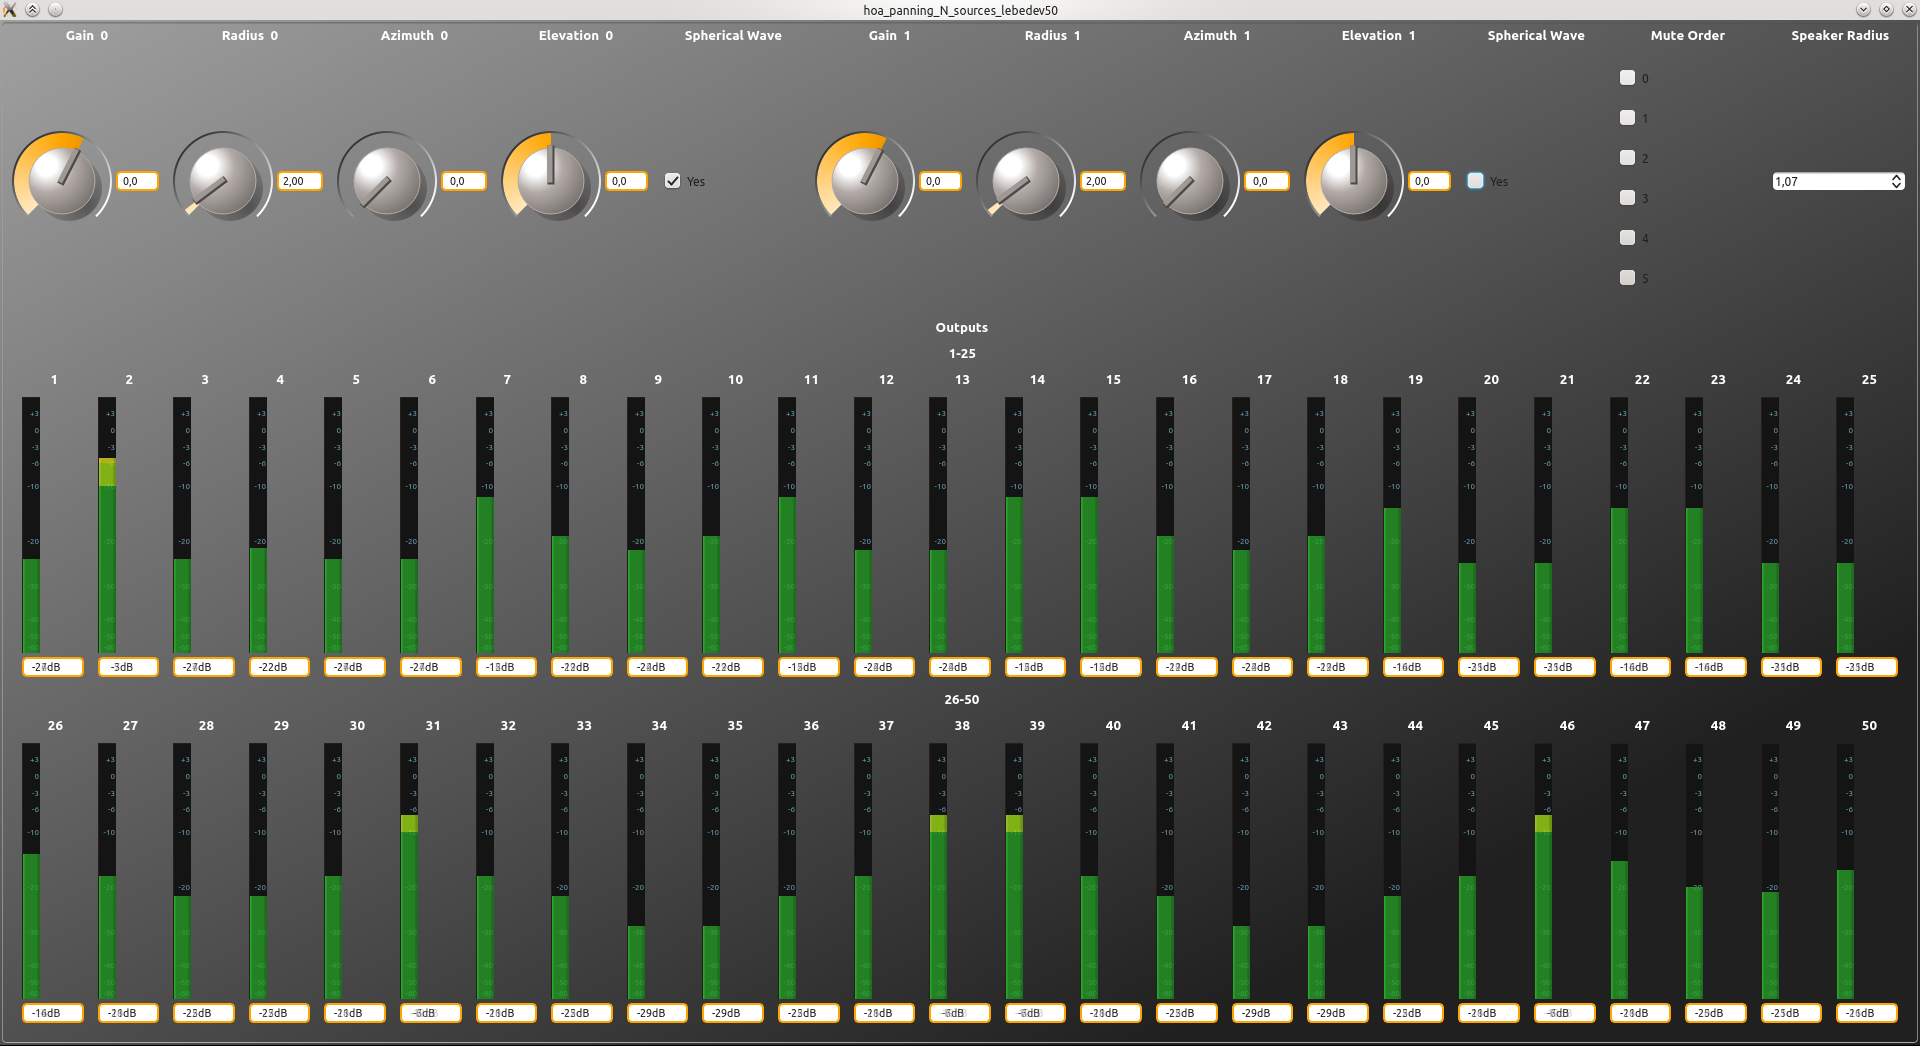
\includegraphics[width=\columnwidth]{hoa_panning_lebedev50.png}
\caption{\lstinline'hoa_panning_lebedev50' plug-in under Linux jack-qt4. The slider 'Outputs Gain' apply a global gain on all outputs (loudspeakers signals). The check-boxes 'Mute Order' allows to mute some Ambisonic orders in the computation of the driving signals. The sliders 'Gain' 'Radius' 'Azimuth' 'Elevation' controls the position and gain of two sources (spherical waves). In order to stabilize the near-field filters for spherical wave synthesis, the input entry 'Speaker Radius' fixes the loudspeaker array radius.}
\label{fig:hoa_panning_lebedev50}
\end{figure}

\pagebreak
\subsubsection{hoa\_mirroring}
The plug-in \lstinline'hoa_mirroring' allows a sound field transformation in Ambisonic domain. Thus, it should be inserted somewhere in between encoding and decoding steps. The sound field is here flipped upside-down, left-right or front-back, or any combination of the above. The tool changes the sign of particular Ambisonic components to realize the transformation \cite{kronlachner2014spatial}. The graphical user interface using \textsc{Faust} Linux jack-qt compiler is shown in Fig.~\ref{fig:hoa_mirroring}. An example of plug-in insertion under Linux jack is shown in Fig.~\ref{fig:hoa_mirroring_claudia}.
\begin{figure}[!ht]
\centering
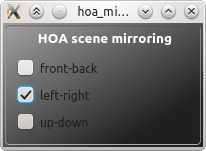
\includegraphics[width=0.3\columnwidth]{hoa_mirroring.png}
\caption{\lstinline'hoa_mirroring' plug-in under Linux jack-qt4. The check-boxes allows to select the mirror transformation : 'left-right', 'front-back' or 'up-down'.}
\label{fig:hoa_mirroring}
\end{figure}
\begin{figure}[!ht]
\centering
\includegraphics[width=0.5\columnwidth]{hoa_mirroring_claudia.png}
\caption{Example of \lstinline'hoa_mirroring' insertion between encoding and decoding steps, i.e. in Ambisonic domain.}
\label{fig:hoa_mirroring_claudia}
\end{figure}

\pagebreak
\subsubsection{hoa\_azimuth\_rotator}
\subsubsection{hoa\_beamforming\_hypercardioid\_to\_mono}
\subsubsection{hoa\_beamforming\_hypercardioid\_to\_hoa}
\subsubsection{hoa\_beamforming\_dirac\_to\_hoa}

\pagebreak
\subsection{Processing}
\subsubsection{Spherical\_VU\_Meter}
\label{sec:processing}
ambitools provides a Spherical VU-Meter developped with \textsc{Processing} language. A screen-shot is shown on Fig.~\ref{fig:spherical_vu_meter}. This tool allows to "see" where the sound energy is in space, instead of using classical in-line VU-Meter. You can zoom, pan and rotate the view of the meter while running. The \textsc{Faust} tools \lstinline'hoa_panning*' and \lstinline'hoa_decoder*' emit \textsc{OSC} messages on port UDP 5511. Those messages drive the spherical VU-Meter rendering in real-time: loudspeakers size and color for the meter, and source position.
\begin{figure}[!ht]
\centering
\includegraphics[width=\columnwidth]{spherical_vu_meter.png}
\caption{\lstinline'Spherical_VU_Meter' for a 50 loudspeaker Lebedev array and two virtual sources. Each loudspeaker is represented as a color ball with size and color proportional to RMS Level in dBFS. A scale in dBFS is displayed on the left of the screen. The virtual sources are represented as red an yellow dots. Their coordinates are displayed in Cartesian and spherical coordinates on the left. A grey manikin is standing in the middle of the array to indicates the front direction.}
\label{fig:spherical_vu_meter}
\end{figure}

\pagebreak
\subsection{Jconvolver}
\subsubsection{jconvolver\_mic*}
\subsubsection{hrir\_lebedev50}
%\section{Examples}
%\subsection{Flys flying around}
%\subsection{Record trajectories with Ardour}
\bibliography{These,ATIAM,Livres}
\bibliographystyle{apalike}

\end{document}
